%\title{Presentation Template}
\documentclass[10pt]{beamer}

\usetheme[progressbar=frametitle]{metropolis}
\usepackage{appendixnumberbeamer}

\usepackage[compatibility=false]{caption}
\usepackage{subcaption}
\usepackage{csquotes}
\usepackage{booktabs}
\usepackage{hyperref}
\usepackage[scale=2]{ccicons}
\usepackage{tikz}
\usepackage{bm}

\usepackage{caption}
\captionsetup{justification=raggedright,singlelinecheck=false}

\usepackage{sidecap}
\sidecaptionvpos{figure}{c}

\usepackage{fontawesome}

\usepackage{footnpag} %reset footnotes at every page

\makeatother
\renewcommand{\thefootnote}{\ifcase\value{footnote}\or*\or
**\or***\or****\fi}
\makeatletter

\usepackage{xmpmulti}
\usepackage{pgffor}
\usepackage{multimedia}
\usepackage{media9}

\graphicspath{{./img/}}

\usepackage{pgfplots}
\usepgfplotslibrary{dateplot}

\usepackage{xspace}
\newcommand{\themename}{\textbf{\textsc{metropolis}}\xspace}

\definecolor{extralightgray}{gray}{0.85}

\title{Learning an Evolvable Genotype-Phenotype Mapping}
\subtitle{GECCO 2018}
\date{July 17, 2018}
\author{Matthew Andres Moreno \newline {\faTwitter} @MorenoMatthewA \newline}
\titlegraphic{\vspace{32ex}\hfill\includegraphics[height=2.5cm]{img/BEACON-logo}}

\usepackage{fix-cm}

\makeatletter\newcommand\HUGE{\@setfontsize\Huge{28}{34}}\makeatother

\begin{document}

\maketitle

% \begin{frame}{Table of contents}
%   \setbeamertemplate{section in toc}[sections numbered]
%   \tableofcontents[hideallsubsections]
% \end{frame}

\section{Evolvability \& Genotype-Phenotype Map}

\begin{frame}{Defining Evolvability}

outcome of mutations

novelty and viability

\end{frame}

\begin{frame}{Evolvability: Novelty}

sketch

\end{frame}

\begin{frame}{Evolvability: Viability}

sketch

\end{frame}

\begin{frame}{Evolvability \& Genotype-Phenotype Map}

when we screw around in here, we want to tend to have certain outcomes here...
hence genotype-phenotype map impacts evolvability!

\end{frame}

\begin{frame}{Evolvable Genotype-Phenotype Maps}

In EC, we define the genotype-phenotype map.

Option A: use direct genotype-phenotype map
\begin{itemize}
\item might suck
\end{itemize}

Option B: use manually-designed genotype-phenotype map
\begin{itemize}
\item labor-intensive
\item might not be great
\end{itemize}

Option C?

\end{frame}

\section{Autoencoders}

\begin{frame}{Pardon the Interruption \dots}

TODO reviewer comment

\end{frame}

\begin{frame}{Autoencoder Intuition}

two superpowers of autoencoders:
\begin{itemize}

\item compression (bottlenecked autoencoder)

\item de-corruption (denoising autoencoder)

\end{itemize}

\end{frame}

\begin{frame}{Autoencoder Intuition: Bottlenecked}

TODO Police Artist 1

\end{frame}

\begin{frame}{Autoencoder Intuition: Bottlenecked}

Why does this work?

\begin{itemize}

\item faces are a \textit{subset} of all possible images
\item detective and witness have seen lots of faces, learned how to describe face

\end{itemize}

\end{frame}

\begin{frame}{Autoencoder Example: Bottlenecked}

face montage

\end{frame}

\begin{frame}{Autoencoder Example: Bottlenecked}

what is a latent-space interpolation?

\end{frame}

\begin{frame}{Autoencoder Intuition: Denoiser}

TODO Police Artist 2

\end{frame}

\begin{frame}{Autoencoder Intuition: Denoiser}

Why does this work?

\begin{itemize}

\item faces are a \textit{subset} of all possible images
\item symmetries, correlations, and certain universal characteristics of faces $\rightarrow$ fix incomplete/corrupted input
\begin{itemize}
\item usually, eye color is same left/right
\item blue eyes correlated with blond hair
\item faces have same general eye-nose-mouth layout
\end{itemize}

\end{itemize}

\end{frame}

\begin{frame}{Autoencoder Intuition: Example}

face reconstruction

\end{frame}

\begin{frame}{Autoencoder Implementation}

How exactly does this all work?

deep learning

(a.k.a. big artificial neural networks tuned with lots of training data)

\end{frame}

\begin{frame}{Autoencoder Implementation}

\begin{figure}
        \begin{subfigure}[b]{0.50\textwidth}
          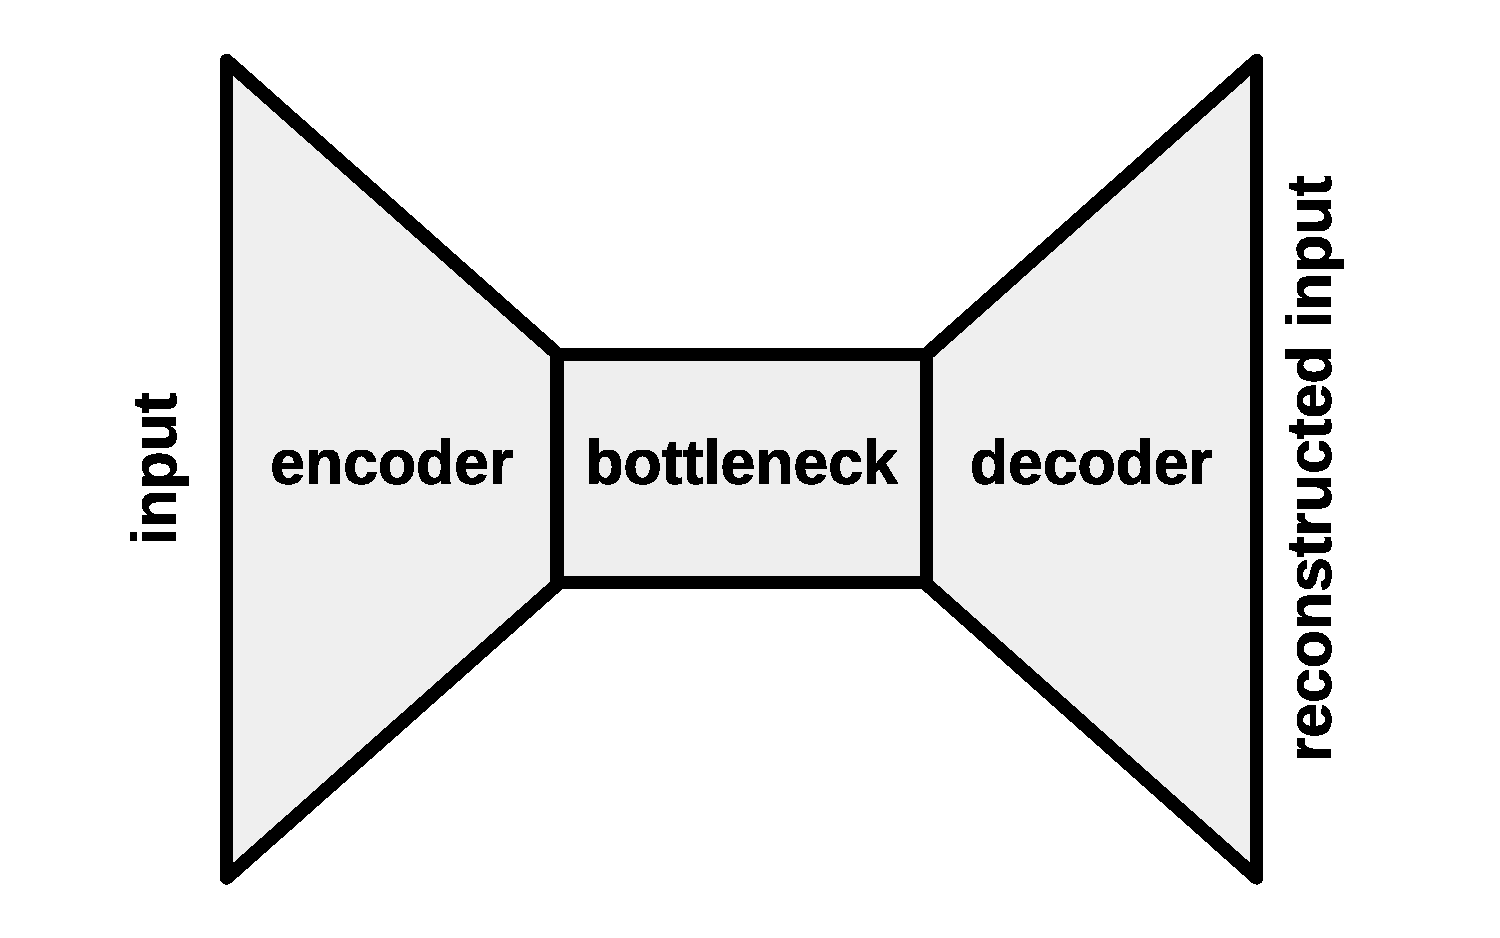
\includegraphics[width=\textwidth]{img/bottleneck}
          \subcaption{bottleneck autoencoder}
          \label{fig:bottleneck}
        \end{subfigure}%
        \begin{subfigure}[b]{0.50\textwidth}
          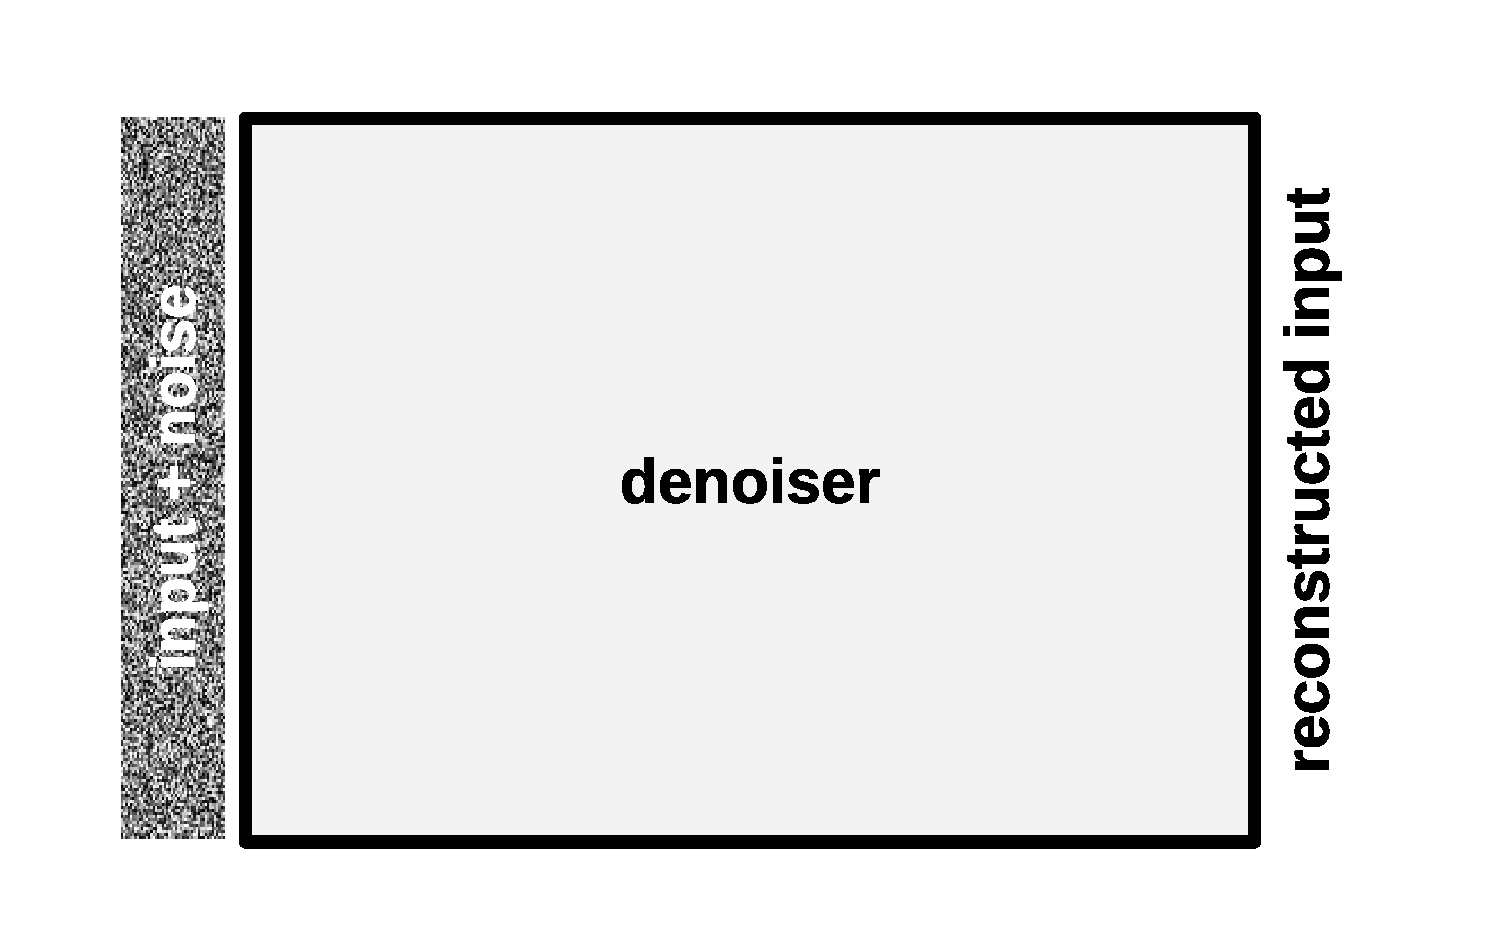
\includegraphics[width=\textwidth]{img/denoiser}
          \subcaption{denoising autoencoder}
          \label{fig:denoiser}
        \end{subfigure}%
        \caption{
          Schematics of bottlenecked a denoising autoencoders.
        }\label{fig:autoencoders}
\end{figure}


\end{frame}

\section{Using Autoencoders to Learn a Genotype-Phenotype Map}

\begin{frame}{Remember This?}
face montage
\end{frame}

\begin{frame}{Bottlenecked G-P Map: Implementation}

\end{frame}

\begin{frame}{Bottlenecked G-P Map: Evolvability}

\end{frame}

\begin{frame}{Remember This?}
face fixups
\end{frame}

\begin{frame}{Denoising G-P Map: Implementation}

\end{frame}

\begin{frame}{Denoising G-P Map: Evolvability}

\end{frame}

\begin{frame}{Autoencoder G-P Maps: Training}

use lots of examples of good solutions
\begin{itemize}
\item evolution with direct encoding
\item evolution with manually-designed indirect encoding
\item maybe they already exist (ex faces)
\end{itemize}

\end{frame}

\section{Experiment: Toy Problem}

\section{Experiment: Scrabble String Problem}

\begin{frame}{Experiment}

reviewer comment on param settings

\end{frame}

\begin{frame}{Denoiser Map Implementation}

\begin{figure}
  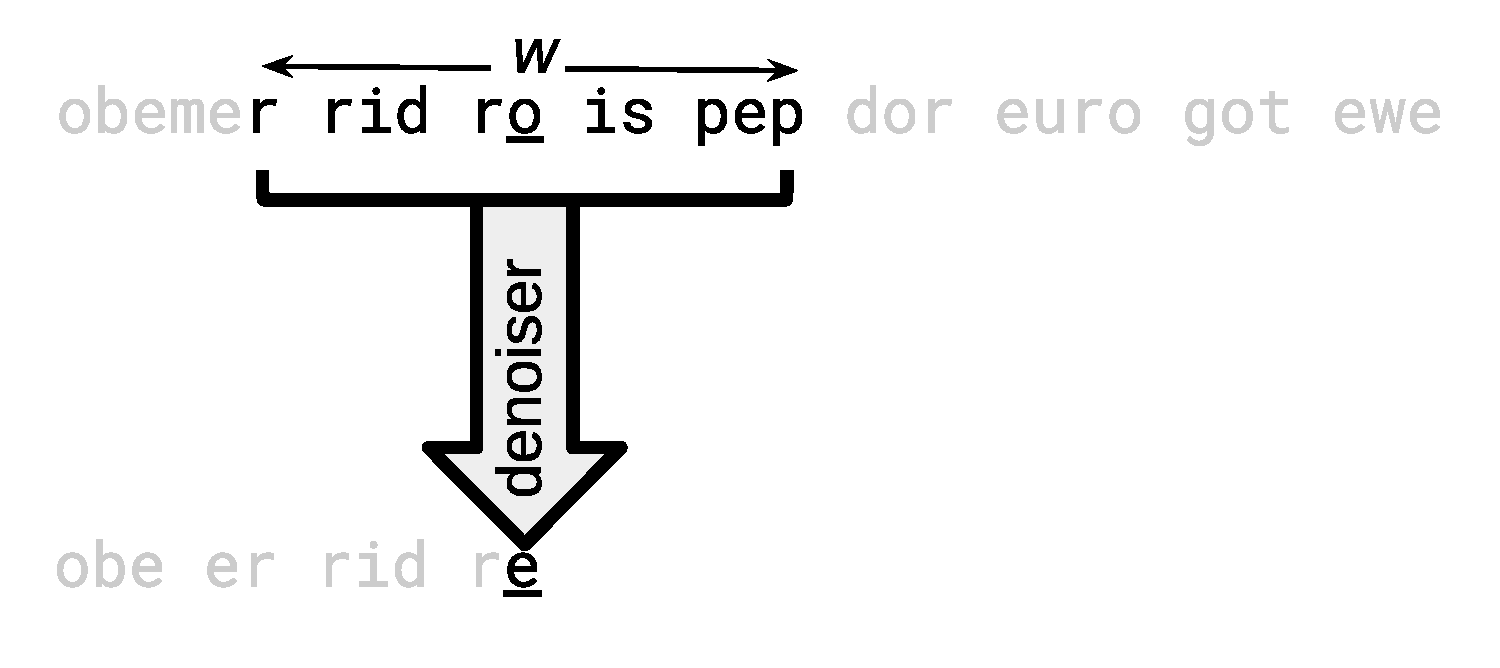
\includegraphics[width=\textwidth]{img/scrabble_denoiser_in_action}
  \caption{
    Illustration of denoising autoencoder in action in the Scrabble domain.
  }\label{fig:scrabble_denoiser_in_action}
\end{figure}


\end{frame}

\begin{frame}{Training Data}

%bold monospaced TODO

\centering \Large

$\downarrow$ evolve word strings $\downarrow$

\dots\texttt{ns fed oxo sob }\dots

$\downarrow$ corrupt letter (sometimes) $\downarrow$

\dots\texttt{ns fed \fbox{o}xo sob }\dots

$\downarrow$ autoencoder guesses original letter $\downarrow$

\dots\texttt{ns fed \fbox{o}xo sob }\dots

$\downarrow$ check guess $\downarrow$

if wrong, adjust autoencoder

\end{frame}

\begin{frame}{Training Data}

%bold monospaced TODO

\centering \Huge

\dots\texttt{ns fed \fbox{o}xo sob }\dots

$\downarrow$

\dots\texttt{ns fed \fbox{o}xo sob }\dots

\end{frame}




\begin{frame}{Intuition: Glorified Spell-Checker}

\centering \Huge

\dots\texttt{la lob ~re as s}\dots

$\downarrow$

\dots\texttt{la lob \fbox{o}re as s}\dots

\end{frame}

\begin{frame}{Intuition: Glorified Spell-Checker}

\centering \Huge

\dots\texttt{lk y ag\fbox{x}r sned }\dots

$\downarrow$

\dots\texttt{lk y ag\fbox{a}r sned }\dots

\end{frame}

%TODO check words

\begin{frame}{Intuition: Glorified Spell-Checker}

\centering \Huge

\dots\texttt{tils r\fbox{a}t ~vow }\dots

$\downarrow$

\dots\texttt{tils r\fbox{t}t ~vow }\dots

\end{frame}

\begin{frame}{Result: Viability under Mutation}

\begin{figure}
  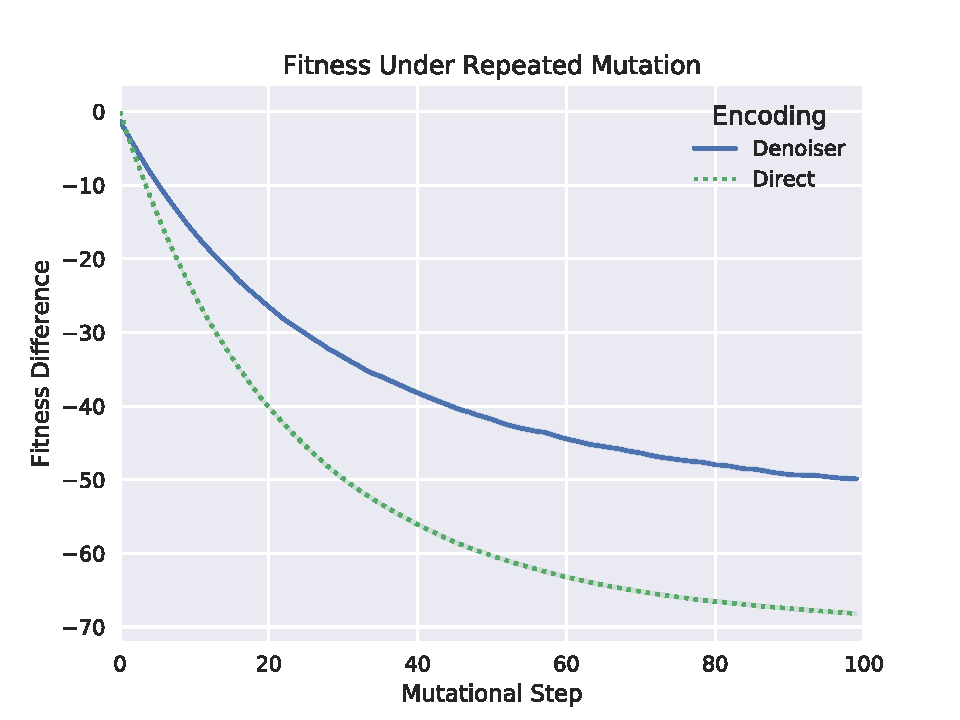
\includegraphics[width=0.8\linewidth]{img/results/scrabble_fit_diff_vs_step}
  \caption{
    Fitness loss by mutational step in the Scrabble string domain.
    Bootstrapped 95\% confidence intervals are shaded along each curve.
    }\label{fig:scrabble_fit_diff_vs_step}
\end{figure}


\end{frame}

\begin{frame}{Result: Novelty under Mutation}

\begin{figure}
  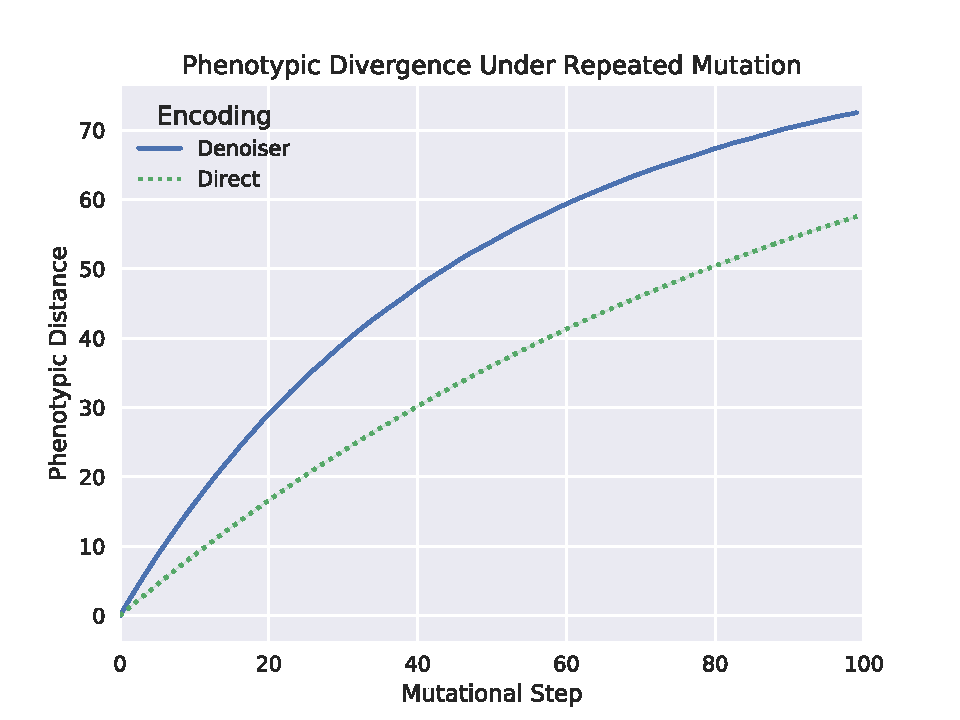
\includegraphics[width=0.85\linewidth]{img/results/scrabble_dist_vs_step}
  \caption{
    Phenotypic divergence by mutational step in the Scrabble string domain.
    Bootstrapped 95\% confidence intervals are shaded along each curve.
  }\label{fig:scrabble_dist_vs_step}
\end{figure}


\end{frame}

\begin{frame}{Result: Fitness}

\begin{figure}
  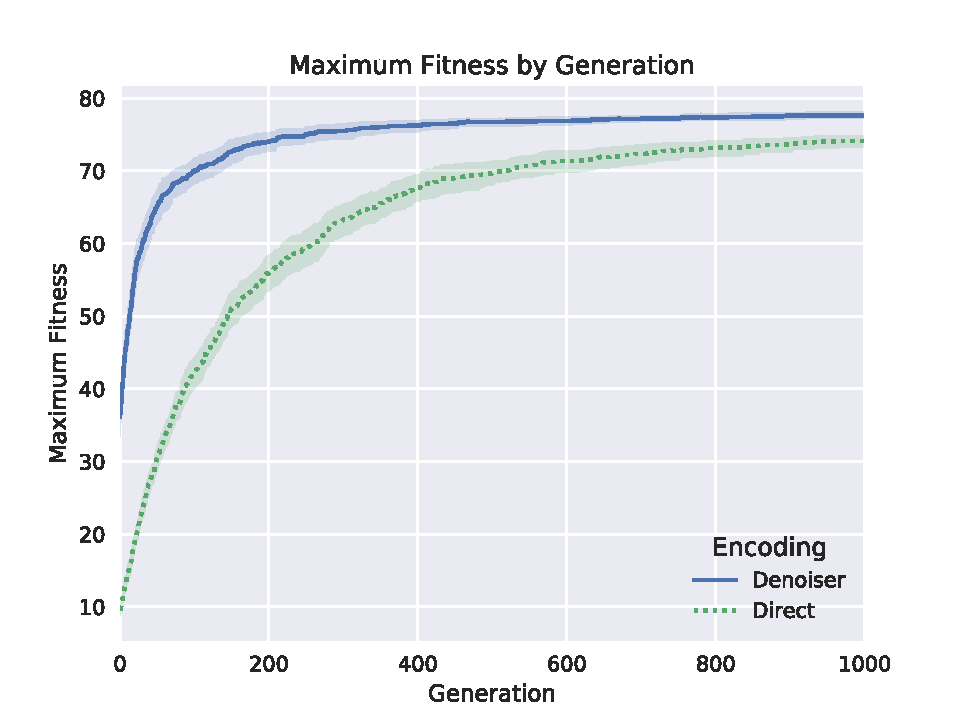
\includegraphics[width=0.8\linewidth]{img/results/scrabble_fit_vs_gen}
  \caption{
    Maximum individual fitness by generation in populations evolving in the Scrabble string domain.
    Bootstrapped 95\% confidence intervals are shaded along each curve.
  }\label{fig:scrabble_fit_vs_gen}
\end{figure}


\end{frame}

\section{Conclusion}

\begin{frame}{Summary}

\end{frame}

\begin{frame}{Challenges (\& Solutions?)}

Unfortunately, autoencoder design and training itself typically
requires skilled human input; AutoMap cannot entirely sidestep the
need for manual labor. Indeed, the question of how to adapt autoen-
coder architecture and training to a less well-understood domain is
nontrivial. For example, questions such as “What should the size
of the bottleneck be for a bottlenecked autoencoder?” or “What
type of noise should a denoising autoencoder be trained with?”
will need to be addressed in any application of AutoMap. It should
also be noted that the success of AutoMap in any problem domain
depends on the computational capacity to generate large amounts
of training data through direct evolution and a willingness to accept
the computational cost of performing a forward pass through the
autoencoder component for each fitness evaluation when evolving
with a learned genotype-phenotype map. Domains where evolu-
tion with pre-existing encodings generate poor solutions, repeated
cycles of autoencoder training and generation of new training data
via evolution might be necessary to yield satisfactory performance.

chicken \& egg: iterative bootstrapping

\end{frame}

\begin{frame}{Next Steps}

demonstrate on more challenging problem

soft-bodied robots?

\end{frame}

\begin{frame}{Next Steps}

put in conversation with ML-evolvability synthesis

citations

call me, beep me, you know how to reach me \dots

or just have some cool ideas and cite me

\end{frame}

\appendix

\begin{frame}{For More Information}

\vspace{1ex}

{\HUGE\url{https://osf.io/n92c7/}}

\vspace{3ex}

\begin{itemize}
\item source code
\item data
\item figures and graphics
\item how-to-replicate tutorial
\item publication
\item slides
\item blog article
\end{itemize}

\end{frame}

\begin{frame}{People}

\vspace{1ex}

\begin{columns}
\begin{column}{0.25\textwidth}
  \centering
  \includegraphics[width=0.7\textwidth,trim={0 15 0 15},clip]{moreno}
\end{column}
\begin{column}{0.75\textwidth}
  \textbf{Matthew Andres Moreno}

  \href{https://twitter.com/MorenoMatthewA}{{\faTwitter} @MorenoMatthewA}

  \href{https://mmore500.github.io}{{\faGlobe} \texttt{https://mmore500.github.io}}

  \href{mailto: mmore500@msu.edu}{{\faEnvelope} \texttt{mmore500@msu.edu}}

\end{column}
\end{columns}

\vspace{1ex}

\begin{columns}
\begin{column}{0.25\textwidth}
  \centering
  \includegraphics[width=0.7\textwidth,trim={0 100 0 50},clip]{banzhaf}
\end{column}

\begin{column}{0.75\textwidth}
  \textbf{Wolfgang Banzhaf}

  \href{http://www.cse.msu.edu/~banzhafw/}{{\faGlobe} \texttt{http://www.cse.msu.edu/\textasciitilde{}banzhafw/}}

  \href{mailto: banzhafw@msu.edu}{{\faEnvelope} \texttt{banzhafw@msu.edu}}

\end{column}
\end{columns}

\vspace{1ex}

\begin{columns}
\begin{column}{0.25\textwidth}
  \centering
  \includegraphics[width=0.7\textwidth]{ofria}
\end{column}

\begin{column}{0.75\textwidth}
  \textbf{Charles Ofria}

  \href{https://twitter.com/CharlesOfria}{{\faTwitter} @CharlesOfria}

  \href{https://ofria.com}{{\faGlobe} \texttt{https://ofria.com}}

  \href{mailto: ofria@msu.edu}{{\faEnvelope} \texttt{ofria@msu.edu}}

\end{column}
\end{columns}

\end{frame}

\begin{frame}{Acknowledgements}
\begin{itemize}
\item Distributed Evolutionary Algorithms for Python
package \cite{fortin2012deap}
\item PyTorch Deep Learning framework \cite{paszke2017pytorch}
\item Open Science Framework via the Center for Open Science
\item computational resources via Michigan State University's Institute for Cyber-Enabled Research
\item computational resources via Google Cloud Compute
\end{itemize}

\vfill

\newcommand{\innerspacer}{0.07\textwidth}
\newcommand{\content}{0.24\textwidth}
\newcommand{\outerspacer}{0.07\textwidth}

\begin{center}
 \begin{columns}
	\begin{column}{\outerspacer}~\end{column}
	 \begin{column}{\content}
		\includegraphics[width=\textwidth]{NSF-logo}
 	\end{column}
  \begin{column}{\innerspacer}~\end{column}
	 \begin{column}{\content}
		\includegraphics[width=\textwidth]{BEACON-logo}
 	\end{column}
  \begin{column}{\innerspacer}~\end{column}
 	\begin{column}{\content}
   \includegraphics[width=0.75\textwidth]{MSU-helmet}
 	\end{column}
 	\begin{column}{\outerspacer}~\end{column}
 \end{columns}
\end{center}

\end{frame}


\begin{frame}[standout]
  Questions?
\end{frame}

\begin{frame}[allowframebreaks]{References}

  \bibliography{bibl}
  \setbeamertemplate{bibliography item}{\insertbiblabel}
  \nocite{*} % Insert publications even if they are not cited in the poster
  \bibliographystyle{apalike}
\end{frame}


\begin{frame}{Scrabble Result: Evolvability Signature}

\begin{figure}
  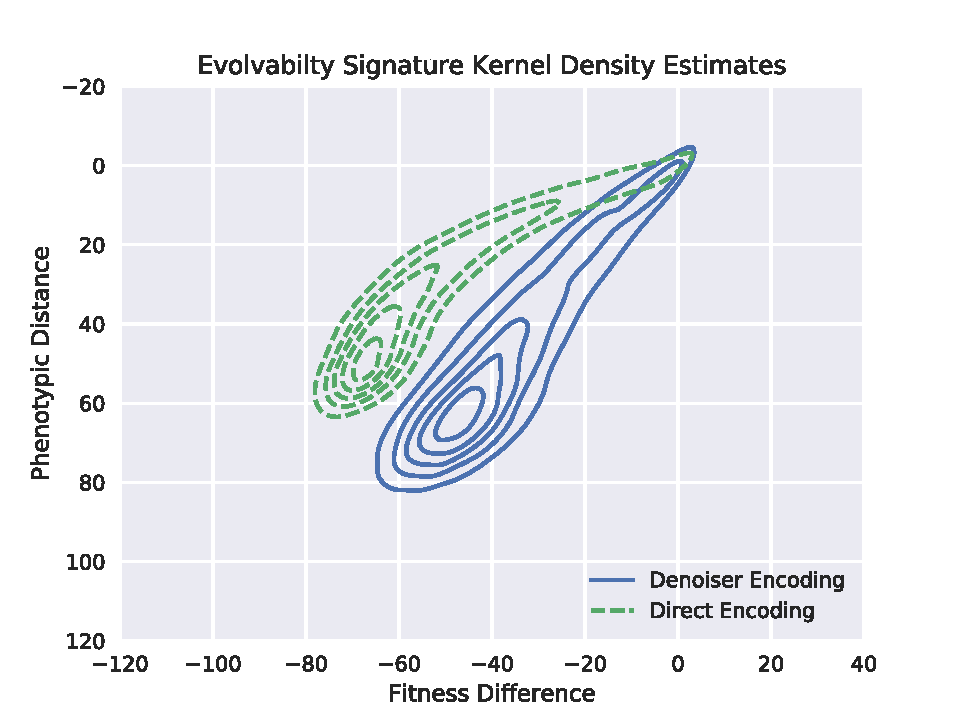
\includegraphics[width=0.8\linewidth]{img/results/scrabble_es_kde}
  \caption{
    Gaussian kernel density estimates for evolvability signatures of direct and indirect encodings in Scrabble string domain.
  }\label{fig:scrabble_es_kde}
\end{figure}


\end{frame}

\begin{frame}{Toy Result: Evolvability Signature}

\begin{figure}
  \begin{subfigure}[b]{0.33\linewidth}
    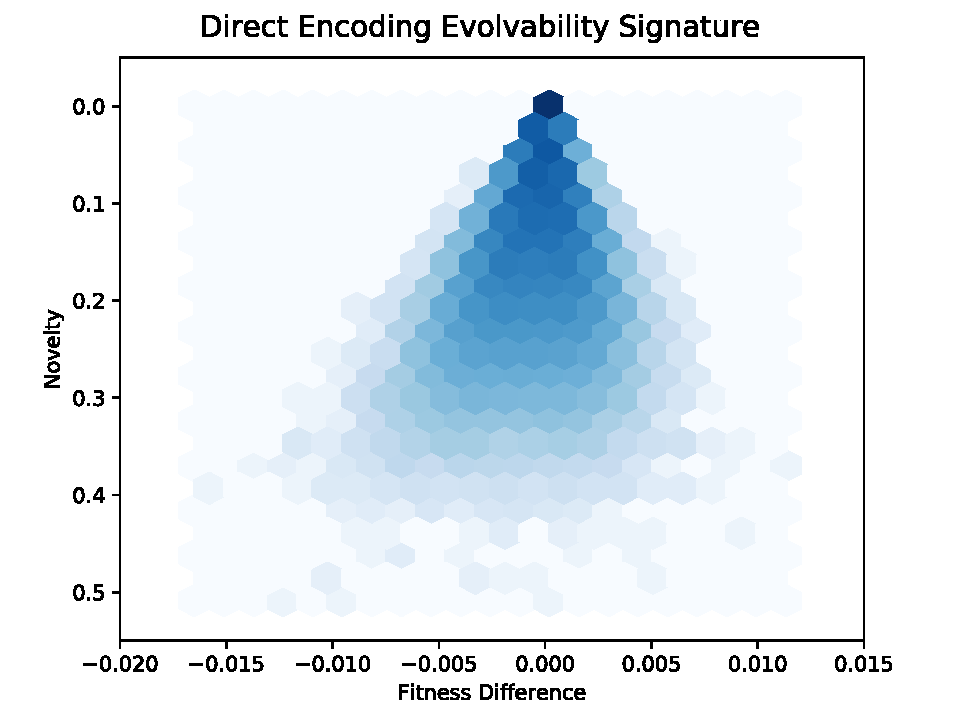
\includegraphics[width=\linewidth]{img/results/direct_es_unscaled}
    \subcaption{
      direct map
    }\label{fig:table_direct_es}
  \end{subfigure}
  \begin{subfigure}[b]{0.33\linewidth}
    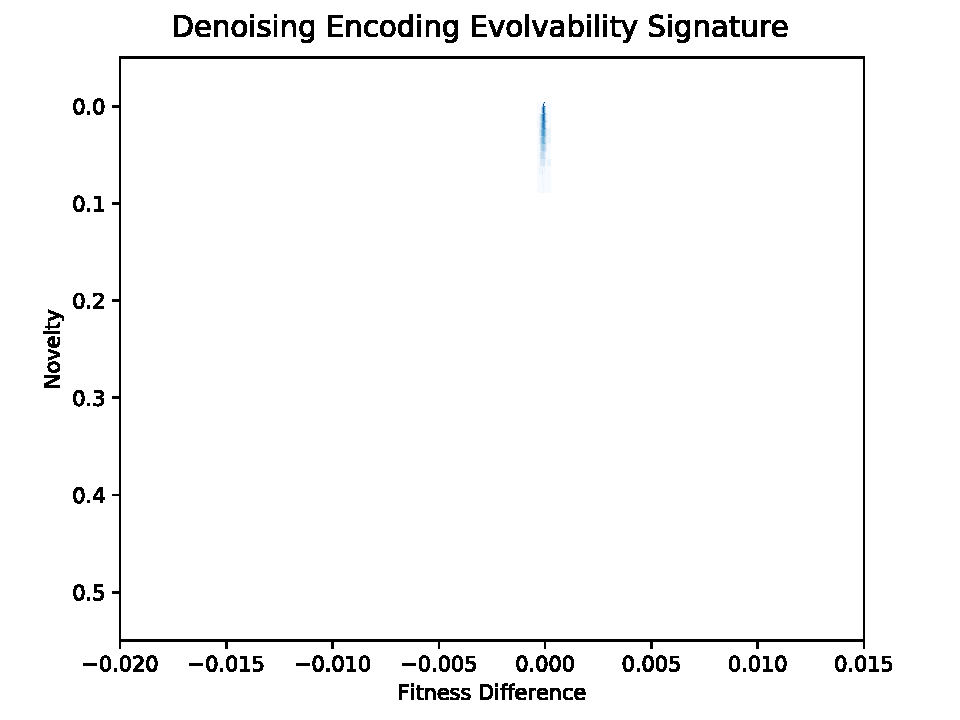
\includegraphics[width=\linewidth]{img/results/noise_es_unscaled}
    \subcaption{
      denoising map
    }\label{fig:table_noise_es}
  \end{subfigure}
  \begin{subfigure}[b]{0.33\linewidth}
    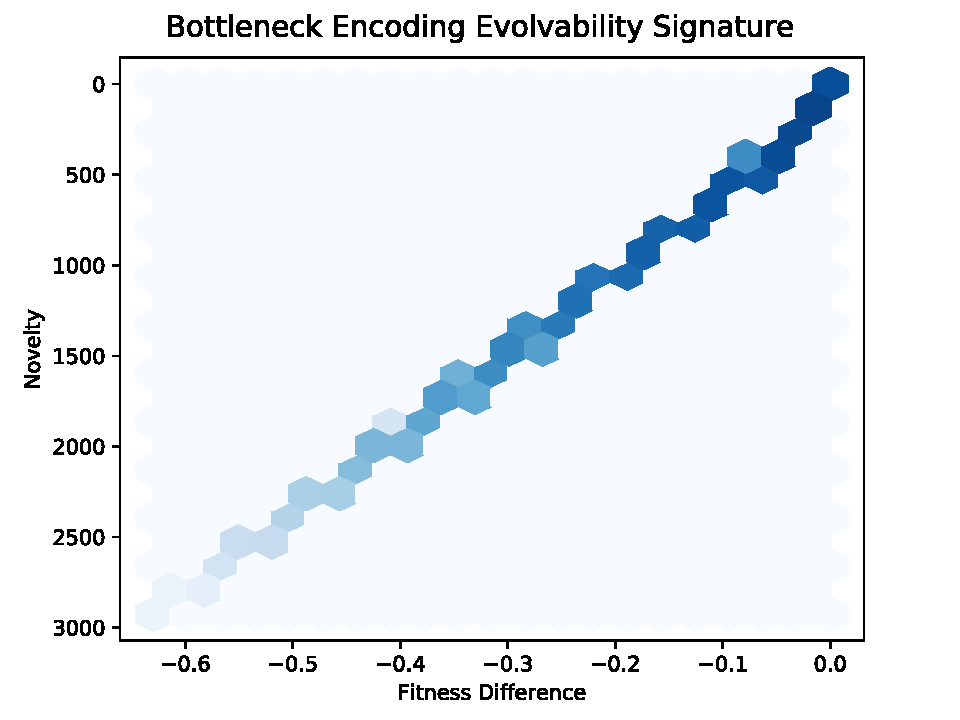
\includegraphics[width=\linewidth]{img/results/bottleneck_es_unscaled}
    \subcaption{
      bottleneck map
    }\label{fig:table_bottleneck_es}
  \end{subfigure}
  \caption{
    Evolvability signatures for three genotype-phenotype maps in the $n$-legged table problem domain.
    Note that subfigure \ref{fig:table_bottleneck_es} is presented with different axis scaling than subfigures \ref{fig:table_direct_es} and \ref{fig:table_noise_es}.
  }\label{fig:all_es}
\end{figure}


\end{frame}

\begin{frame}{Evolutionary Algorithm Parameters: Toy Problem}

\begin{itemize}
\item population size: 300
\item tournament selection: $k = 5$
\item crossover: two-point, two-parent, $p = 0.5$
\item mutation: site-wise Gaussian perturbation
\begin{itemize}
\item training data, evolvability-signature experiments: $\mu = 0$, $\sigma = 0.1$, per-individual
probability = 0.2, per-site probability = 0.01
\item response-to-selection experiments: $\mu = 0$, $\sigma = 0.1$, per-individual probability = 0.2, per-site probability = 0.2 %TODO check this
\footnote{for the bottleneck map, a per-site probability of 1 was employed}
\end{itemize}
\end{itemize}

\end{frame}

\begin{frame}{Denoising Autoencoder Hyperparameters: Toy Problem}

\begin{itemize}
\item 100-to-100 fully-connected linear layer without bias
\item trained for 2500 epochs by stochastic gradient descent
\item learning rate: $10^{−4}$
\item momentum: 0.9
\item batch size: 2048
\item model parameters initialized uniformly between 0.005 and 0.015
\item model parameters clamped in the range (0, 1
\item during the training process, Gaussian
  noise with $\mu = 0$, $\sigma = 0.025$ applied to input
\item loss: mean square error of the difference between the original phenotype the reconstructed phenotype
\end{itemize}

\end{frame}

\begin{frame}{Evolutionary Algorithm Parameters: Scrabble Problem}

TODO

\end{frame}


\end{document}
